\begin{figure}
	\centering
	\pgfplotsset{every axis legend/.append style={
		at={(1.05,0.5)},
		anchor=west}}
	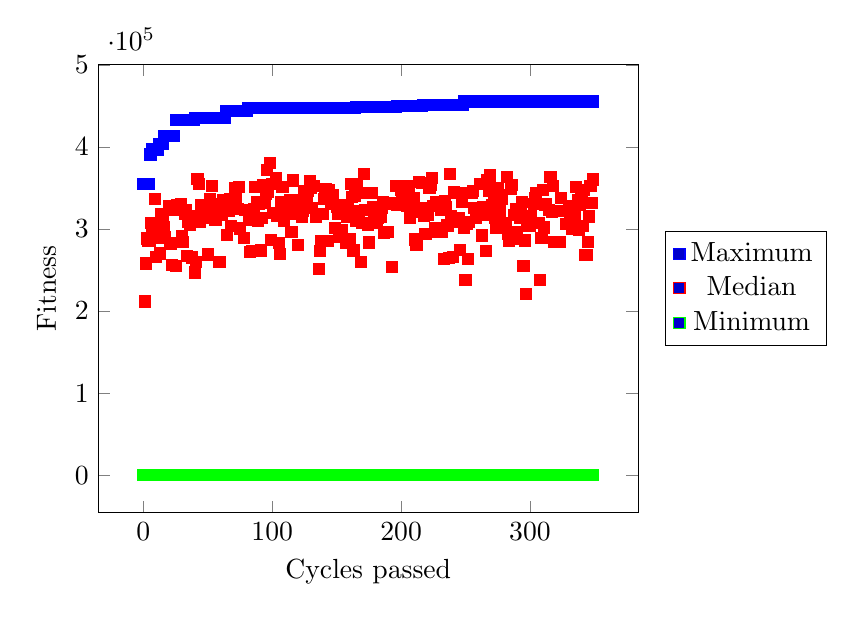
\begin{tikzpicture}
		\begin{axis}[
			xlabel=Cycles passed,
			ylabel=Fitness,
			scatter/classes={
				max={mark=square*,blue},
				med={mark=square*,red},
				min={mark=square*,green}
				}
            ]
            
\addplot+[scatter,only marks,scatter src=explicit symbolic]table[meta=label] {
x y label
0 354680 max
1 354680 max
2 354680 max
3 354680 max
4 354680 max
5 390664 max
6 390664 max
7 396776 max
8 396776 max
9 396776 max
10 396776 max
11 396776 max
12 403788 max
13 403788 max
14 403788 max
15 403788 max
16 412789 max
17 412789 max
18 412789 max
19 412789 max
20 412789 max
21 412789 max
22 412789 max
23 412789 max
24 412789 max
25 433180 max
26 433180 max
27 433180 max
28 433180 max
29 433180 max
30 433180 max
31 433180 max
32 433180 max
33 433180 max
34 433180 max
35 433180 max
36 433180 max
37 433180 max
38 433180 max
39 433180 max
40 435280 max
41 435280 max
42 435280 max
43 435280 max
44 435280 max
45 435280 max
46 435280 max
47 435280 max
48 435280 max
49 435280 max
50 435280 max
51 435280 max
52 435280 max
53 435280 max
54 435280 max
55 435280 max
56 435280 max
57 435280 max
58 435280 max
59 435280 max
60 435280 max
61 435280 max
62 435280 max
63 435280 max
64 443364 max
65 443364 max
66 443364 max
67 443364 max
68 443364 max
69 443364 max
70 443364 max
71 443364 max
72 443364 max
73 443364 max
74 443364 max
75 443364 max
76 443364 max
77 443364 max
78 443364 max
79 443364 max
80 443364 max
81 447418 max
82 447418 max
83 447418 max
84 447418 max
85 447418 max
86 447418 max
87 447418 max
88 447418 max
89 447418 max
90 447418 max
91 447418 max
92 447418 max
93 447418 max
94 447418 max
95 447418 max
96 447418 max
97 447418 max
98 447418 max
99 447418 max
100 447418 max
101 447418 max
102 447418 max
103 447418 max
104 447418 max
105 447418 max
106 447418 max
107 447418 max
108 447418 max
109 447418 max
110 447418 max
111 447418 max
112 447418 max
113 447418 max
114 447418 max
115 447418 max
116 447418 max
117 447418 max
118 447418 max
119 447418 max
120 447418 max
121 447418 max
122 447418 max
123 447418 max
124 447418 max
125 447418 max
126 447418 max
127 447418 max
128 447418 max
129 447418 max
130 447418 max
131 447418 max
132 447418 max
133 447418 max
134 447418 max
135 447418 max
136 447418 max
137 447418 max
138 447418 max
139 447418 max
140 447418 max
141 447418 max
142 447418 max
143 447418 max
144 447418 max
145 447418 max
146 447418 max
147 447418 max
148 447418 max
149 447418 max
150 447418 max
151 447418 max
152 447810 max
153 447810 max
154 447810 max
155 447810 max
156 447810 max
157 447810 max
158 447810 max
159 447810 max
160 447810 max
161 447810 max
162 447810 max
163 447810 max
164 447810 max
165 448617 max
166 448617 max
167 448617 max
168 448617 max
169 448617 max
170 448617 max
171 448617 max
172 448617 max
173 448617 max
174 448617 max
175 448617 max
176 448617 max
177 448617 max
178 448617 max
179 448617 max
180 448617 max
181 448617 max
182 448617 max
183 448617 max
184 448617 max
185 448617 max
186 448617 max
187 448617 max
188 448617 max
189 448617 max
190 448617 max
191 448617 max
192 448617 max
193 448617 max
194 448617 max
195 448617 max
196 448617 max
197 449395 max
198 449395 max
199 449395 max
200 449395 max
201 449395 max
202 449395 max
203 449395 max
204 449395 max
205 449395 max
206 449395 max
207 449395 max
208 449395 max
209 449395 max
210 449395 max
211 449395 max
212 449395 max
213 449395 max
214 449442 max
215 449442 max
216 449442 max
217 450547 max
218 450547 max
219 450547 max
220 450547 max
221 450547 max
222 450547 max
223 450547 max
224 450547 max
225 450594 max
226 450594 max
227 450594 max
228 450594 max
229 450594 max
230 450594 max
231 450594 max
232 450594 max
233 450594 max
234 450594 max
235 450594 max
236 450594 max
237 450594 max
238 450594 max
239 450594 max
240 450594 max
241 450594 max
242 450594 max
243 450594 max
244 450594 max
245 450594 max
246 450594 max
247 450594 max
248 450594 max
249 455224 max
250 455224 max
251 455224 max
252 455224 max
253 455224 max
254 455224 max
255 455224 max
256 455224 max
257 455224 max
258 455224 max
259 455224 max
260 455224 max
261 455224 max
262 455224 max
263 455224 max
264 455224 max
265 455224 max
266 455224 max
267 455224 max
268 455224 max
269 455224 max
270 455224 max
271 455224 max
272 455224 max
273 455224 max
274 455224 max
275 455224 max
276 455224 max
277 455224 max
278 455224 max
279 455224 max
280 455224 max
281 455224 max
282 455224 max
283 455224 max
284 455224 max
285 455224 max
286 455224 max
287 455224 max
288 455224 max
289 455224 max
290 455224 max
291 455224 max
292 455224 max
293 455224 max
294 455224 max
295 455224 max
296 455224 max
297 455224 max
298 455224 max
299 455224 max
300 455224 max
301 455224 max
302 455224 max
303 455224 max
304 455224 max
305 455224 max
306 455224 max
307 455224 max
308 455224 max
309 455224 max
310 455224 max
311 455224 max
312 455224 max
313 455224 max
314 455224 max
315 455224 max
316 455224 max
317 455224 max
318 455224 max
319 455224 max
320 455224 max
321 455224 max
322 455224 max
323 455224 max
324 455224 max
325 455224 max
326 455224 max
327 455224 max
328 455224 max
329 455224 max
330 455224 max
331 455224 max
332 455224 max
333 455224 max
334 455224 max
335 455224 max
336 455224 max
337 455224 max
338 455224 max
339 455224 max
340 455224 max
341 455224 max
342 455224 max
343 455224 max
344 455224 max
345 455224 max
346 455224 max
347 455224 max
348 455224 max
349 455224 max
};
\addplot+[scatter,only marks,scatter src=explicit symbolic]table[meta=label] {
x y label
0 0 med
1 211699 med
2 257852 med
3 288415 med
4 285891 med
5 285040 med
6 307498 med
7 303793 med
8 302051 med
9 336141 med
10 265379 med
11 288994 med
12 293017 med
13 270079 med
14 318206 med
15 314122 med
16 302052 med
17 289715 med
18 0 med
19 0 med
20 328222 med
21 282179 med
22 256481 med
23 323417 med
24 0 med
25 254478 med
26 328543 med
27 327296 med
28 326165 med
29 329800 med
30 291460 med
31 284028 med
32 318130 med
33 322482 med
34 266980 med
35 309091 med
36 305234 med
37 312794 med
38 265272 med
39 316200 med
40 246915 med
41 259286 med
42 360626 med
43 354607 med
44 308660 med
45 329607 med
46 326342 med
47 317386 med
48 0 med
49 313123 med
50 268850 med
51 319782 med
52 336937 med
53 352685 med
54 329761 med
55 312868 med
56 311359 med
57 324762 med
58 0 med
59 260191 med
60 322595 med
61 317170 med
62 335027 med
63 0 med
64 323896 med
65 292589 med
66 321958 med
67 336464 med
68 303504 med
69 325658 med
70 332248 med
71 349668 med
72 335874 med
73 324335 med
74 351481 med
75 300578 med
76 0 med
77 0 med
78 289155 med
79 322986 med
80 0 med
81 0 med
82 311244 med
83 272157 med
84 272882 med
85 311652 med
86 324178 med
87 351385 med
88 332683 med
89 309591 med
90 330401 med
91 273772 med
92 313019 med
93 353679 med
94 331329 med
95 342899 med
96 371871 med
97 344792 med
98 380465 med
99 286071 med
100 354641 med
101 319144 med
102 0 med
103 362110 med
104 315921 med
105 283051 med
106 269878 med
107 332750 med
108 350724 med
109 309680 med
110 333235 med
111 328404 med
112 318873 med
113 326750 med
114 335405 med
115 296498 med
116 359041 med
117 322553 med
118 335187 med
119 318712 med
120 280281 med
121 0 med
122 0 med
123 314834 med
124 322474 med
125 345724 med
126 327763 med
127 331264 med
128 346662 med
129 358321 med
130 350233 med
131 325400 med
132 352242 med
133 0 med
134 315006 med
135 317810 med
136 250742 med
137 273011 med
138 285470 med
139 318549 med
140 336896 med
141 347617 med
142 348453 med
143 285091 med
144 346802 med
145 336207 med
146 330375 med
147 341497 med
148 0 med
149 301333 med
150 327356 med
151 318154 med
152 290258 med
153 329508 med
154 298411 med
155 320923 med
156 321093 med
157 283076 med
158 314129 med
159 324667 med
160 287125 med
161 354489 med
162 338838 med
163 273634 med
164 339667 med
165 309217 med
166 354392 med
167 322276 med
168 343332 med
169 259276 med
170 307100 med
171 367416 med
172 323161 med
173 343336 med
174 305503 med
175 283488 med
176 306929 med
177 343799 med
178 327021 med
179 314049 med
180 322325 med
181 306859 med
182 313699 med
183 324145 med
184 314121 med
185 325329 med
186 333240 med
187 294788 med
188 0 med
189 0 med
190 295847 med
191 330732 med
192 0 med
193 253140 med
194 331421 med
195 0 med
196 352635 med
197 329153 med
198 0 med
199 0 med
200 347300 med
201 337142 med
202 351634 med
203 341897 med
204 0 med
205 328496 med
206 351957 med
207 313260 med
208 336930 med
209 332540 med
210 337909 med
211 287113 med
212 280179 med
213 323917 med
214 357643 med
215 320949 med
216 355526 med
217 325258 med
218 315844 med
219 294106 med
220 322413 med
221 317030 med
222 350275 med
223 353321 med
224 362071 med
225 327594 med
226 300911 med
227 332889 med
228 296632 med
229 0 med
230 0 med
231 322874 med
232 296086 med
233 263362 med
234 333811 med
235 326915 med
236 304221 med
237 264371 med
238 366900 med
239 316148 med
240 265939 med
241 344436 med
242 308785 med
243 0 med
244 0 med
245 313303 med
246 274649 med
247 333320 med
248 343317 med
249 301070 med
250 237349 med
251 306156 med
252 263579 med
253 308620 med
254 0 med
255 344183 med
256 346115 med
257 325982 med
258 313155 med
259 319626 med
260 0 med
261 355008 med
262 0 med
263 291991 med
264 326758 med
265 317182 med
266 273238 med
267 359896 med
268 346850 med
269 365035 med
270 319860 med
271 328719 med
272 337036 med
273 313107 med
274 301233 med
275 350291 med
276 341462 med
277 322418 med
278 336469 med
279 0 med
280 0 med
281 307469 med
282 363612 med
283 293661 med
284 284985 med
285 349338 med
286 353902 med
287 288116 med
288 316666 med
289 323950 med
290 296233 med
291 0 med
292 313726 med
293 321381 med
294 332609 med
295 255213 med
296 285968 med
297 220965 med
298 304162 med
299 313977 med
300 304184 med
301 315584 med
302 0 med
303 330535 med
304 337051 med
305 343454 med
306 330004 med
307 307142 med
308 237350 med
309 288841 med
310 347588 med
311 301712 med
312 329757 med
313 0 med
314 0 med
315 322675 med
316 363359 med
317 321314 med
318 352183 med
319 283717 med
320 0 med
321 0 med
322 0 med
323 283704 med
324 338074 med
325 321515 med
326 0 med
327 0 med
328 306148 med
329 0 med
330 328453 med
331 312668 med
332 308933 med
333 300194 med
334 326709 med
335 317408 med
336 351398 med
337 335545 med
338 298950 med
339 328767 med
340 343406 med
341 303460 med
342 347043 med
343 268501 med
344 268011 med
345 284296 med
346 315097 med
347 352591 med
348 331572 med
349 360171 med
};
\addplot+[scatter,only marks,scatter src=explicit symbolic]table[meta=label] {
x y label
0 0 min
1 0 min
2 0 min
3 0 min
4 0 min
5 0 min
6 0 min
7 0 min
8 0 min
9 0 min
10 0 min
11 0 min
12 0 min
13 0 min
14 0 min
15 0 min
16 0 min
17 0 min
18 0 min
19 0 min
20 0 min
21 0 min
22 0 min
23 0 min
24 0 min
25 0 min
26 0 min
27 0 min
28 0 min
29 0 min
30 0 min
31 0 min
32 0 min
33 0 min
34 0 min
35 0 min
36 0 min
37 0 min
38 0 min
39 0 min
40 0 min
41 0 min
42 0 min
43 0 min
44 0 min
45 0 min
46 0 min
47 0 min
48 0 min
49 0 min
50 0 min
51 0 min
52 0 min
53 0 min
54 0 min
55 0 min
56 0 min
57 0 min
58 0 min
59 0 min
60 0 min
61 0 min
62 0 min
63 0 min
64 0 min
65 0 min
66 0 min
67 0 min
68 0 min
69 0 min
70 0 min
71 0 min
72 0 min
73 0 min
74 0 min
75 0 min
76 0 min
77 0 min
78 0 min
79 0 min
80 0 min
81 0 min
82 0 min
83 0 min
84 0 min
85 0 min
86 0 min
87 0 min
88 0 min
89 0 min
90 0 min
91 0 min
92 0 min
93 0 min
94 0 min
95 0 min
96 0 min
97 0 min
98 0 min
99 0 min
100 0 min
101 0 min
102 0 min
103 0 min
104 0 min
105 0 min
106 0 min
107 0 min
108 0 min
109 0 min
110 0 min
111 0 min
112 0 min
113 0 min
114 0 min
115 0 min
116 0 min
117 0 min
118 0 min
119 0 min
120 0 min
121 0 min
122 0 min
123 0 min
124 0 min
125 0 min
126 0 min
127 0 min
128 0 min
129 0 min
130 0 min
131 0 min
132 0 min
133 0 min
134 0 min
135 0 min
136 0 min
137 0 min
138 0 min
139 0 min
140 0 min
141 0 min
142 0 min
143 0 min
144 0 min
145 0 min
146 0 min
147 0 min
148 0 min
149 0 min
150 0 min
151 0 min
152 0 min
153 0 min
154 0 min
155 0 min
156 0 min
157 0 min
158 0 min
159 0 min
160 0 min
161 0 min
162 0 min
163 0 min
164 0 min
165 0 min
166 0 min
167 0 min
168 0 min
169 0 min
170 0 min
171 0 min
172 0 min
173 0 min
174 0 min
175 0 min
176 0 min
177 0 min
178 0 min
179 0 min
180 0 min
181 0 min
182 0 min
183 0 min
184 0 min
185 0 min
186 0 min
187 0 min
188 0 min
189 0 min
190 0 min
191 0 min
192 0 min
193 0 min
194 0 min
195 0 min
196 0 min
197 0 min
198 0 min
199 0 min
200 0 min
201 0 min
202 0 min
203 0 min
204 0 min
205 0 min
206 0 min
207 0 min
208 0 min
209 0 min
210 0 min
211 0 min
212 0 min
213 0 min
214 0 min
215 0 min
216 0 min
217 0 min
218 0 min
219 0 min
220 0 min
221 0 min
222 0 min
223 0 min
224 0 min
225 0 min
226 0 min
227 0 min
228 0 min
229 0 min
230 0 min
231 0 min
232 0 min
233 0 min
234 0 min
235 0 min
236 0 min
237 0 min
238 0 min
239 0 min
240 0 min
241 0 min
242 0 min
243 0 min
244 0 min
245 0 min
246 0 min
247 0 min
248 0 min
249 0 min
250 0 min
251 0 min
252 0 min
253 0 min
254 0 min
255 0 min
256 0 min
257 0 min
258 0 min
259 0 min
260 0 min
261 0 min
262 0 min
263 0 min
264 0 min
265 0 min
266 0 min
267 0 min
268 0 min
269 0 min
270 0 min
271 0 min
272 0 min
273 0 min
274 0 min
275 0 min
276 0 min
277 0 min
278 0 min
279 0 min
280 0 min
281 0 min
282 0 min
283 0 min
284 0 min
285 0 min
286 0 min
287 0 min
288 0 min
289 0 min
290 0 min
291 0 min
292 0 min
293 0 min
294 0 min
295 0 min
296 0 min
297 0 min
298 0 min
299 0 min
300 0 min
301 0 min
302 0 min
303 0 min
304 0 min
305 0 min
306 0 min
307 0 min
308 0 min
309 0 min
310 0 min
311 0 min
312 0 min
313 0 min
314 0 min
315 0 min
316 0 min
317 0 min
318 0 min
319 0 min
320 0 min
321 0 min
322 0 min
323 0 min
324 0 min
325 0 min
326 0 min
327 0 min
328 0 min
329 0 min
330 0 min
331 0 min
332 0 min
333 0 min
334 0 min
335 0 min
336 0 min
337 0 min
338 0 min
339 0 min
340 0 min
341 0 min
342 0 min
343 0 min
344 0 min
345 0 min
346 0 min
347 0 min
348 0 min
349 0 min
};

			\addlegendentry{Maximum}
			\addlegendentry{Median}
			\addlegendentry{Minimum}
		\end{axis}
	\end{tikzpicture}
	\caption{Detail of genetic algorithm on balanced data with 35 elements in set}
\label{plot:genProfile35}
\end{figure}
